
%(BEGIN_QUESTION)
% Copyright 2010, Tony R. Kuphaldt, released under the Creative Commons Attribution License (v 1.0)
% This means you may do almost anything with this work of mine, so long as you give me proper credit

Suppose you decide to start your own whipped-cream manufacturing business, using a PLC to control the cream ``whipping'' machine.  This is a batch process, where the PLC fills the mixing tank with a load of raw cream, proceeds to whip the cream by spinning the paddlewheel a certain number of times, and then empties the tank to get ready to process another batch.  The paddlewheel's rotation is critical -- if the cream is churned excessively by the paddlewheel (i.e. too many rotations), it turns into {\it butter} instead of whipped cream.  The PLC is programmed to count the number of shaft rotations, and stop the whipping process when the required number of rotations is reached:

$$\includegraphics[width=15.5cm]{i01885x01.eps}$$

After working properly for several months, one of your maintenance technicians decides to re-adjust the proximity sensor near the motor shaft, and accidently moves it too far away from the motor shaft to detect the shaft's rotation like it is supposed to.

\vskip 10pt

Describe the effect this mis-adjustment will have on the operation of your whipped-cream process.

\vskip 50pt

Secondly, describe a way you could program the PLC to avoid this problem even in the event of a mis-adjusted proximity sensor.

\vfil \eject

\underbar{file i01885}
%(END_QUESTION)





%(BEGIN_ANSWER)

With the sensor mis-adjusted, the PLC will not know when to stop, and it will whip the cream into butter!

\vskip 10pt

A ``fix'' for this problem is to include a counter instruction in the PLC's programming, such that the paddlewheel is limited in run-time, to avoid whipping the cream into butter.  Alternatively, a timer instruction could be used to measure how many turns of the paddlewheel occur in the first few seconds of operation: if no turns are detected, the system shuts off with an alarm.

%(END_ANSWER)





%(BEGIN_NOTES)

{\bf This question is intended for exams only and not worksheets!}.

%(END_NOTES)

